%============================================================================%
%
%	DOCUMENT DEFINITION
%
%============================================================================%

%we use article class because we want to fully customize the page and don't use a cv template
\documentclass[spanish,10.5pt,A4]{article}	

%----------------------------------------------------------------------------------------
%	ENCODING
%----------------------------------------------------------------------------------------

% we use utf8 since we want to build from any machine
\usepackage[utf8]{inputenc}

%----------------------------------------------------------------------------------------
%	LOGIC
%----------------------------------------------------------------------------------------

% provides \isempty test
\usepackage{xstring, xifthen}

%----------------------------------------------------------------------------------------
%	FONT BASICS
%----------------------------------------------------------------------------------------

% some tex-live fonts - choose your own

\usepackage[spanish]{babel}

%\usepackage[defaultsans]{droidsans}
%\usepackage[default]{comfortaa}
%\usepackage{cmbright}
%\usepackage[default]{raleway}
%\usepackage{fetamont}
%\usepackage[default]{gillius}
%\usepackage[light,math]{iwona}
%\usepackage[thin]{roboto} 

% set font default
% \renewcommand*\familydefault{\sfdefault} 	
\usepackage[T1]{fontenc}

% more font size definitions
\usepackage{moresize}

\usepackage{setspace}
\renewcommand{\baselinestretch}{1.25}

%----------------------------------------------------------------------------------------
%	FONT AWESOME ICONS
%---------------------------------------------------------------------------------------- 

% include the fontawesome icon set
\usepackage{fontawesome}

% use to vertically center content
% credits to: http://tex.stackexchange.com/questions/7219/how-to-vertically-center-two-images-next-to-each-other
\newcommand{\vcenteredinclude}[1]{\begingroup
\setbox0=\hbox{\includegraphics{#1}}%
\parbox{\wd0}{\box0}\endgroup}

% use to vertically center content
\newcommand*{\vcenteredhbox}[1]{\begingroup
\setbox0=\hbox{#1}\parbox{\wd0}{\box0}\endgroup}

% icon shortcut
\newcommand{\icon}[3] { 							
	\makebox(#2, #2){\textcolor{maincol}{\csname fa#1\endcsname}}
}	

% icon with text shortcut
\newcommand{\icontext}[4]{ 						
	\vcenteredhbox{\icon{#1}{#2}{#3}}  \hspace{0.5pt}  \parbox{0.9\mpwidth}{\textcolor{#4}{#3}}
}

% icon with website url
\newcommand{\iconhref}[5]{ 						
    \vcenteredhbox{\icon{#1}{#2}{#5}}  \hspace{0.5pt} \href{#4}{\textcolor{#5}{#3}}
}

% icon with email link
\newcommand{\iconemail}[5]{ 						
    \vcenteredhbox{\icon{#1}{#2}{#5}}  \hspace{0.5pt} \href{mailto:#4}{\textcolor{#5}{#3}}
}

%----------------------------------------------------------------------------------------
%	PAGE LAYOUT  DEFINITIONS
%----------------------------------------------------------------------------------------

% page outer frames (debug-only)
% \usepackage{showframe}		

\usepackage{ragged2e}

% we use paracol to display breakable two columns
\usepackage{paracol}

% define page styles using geometry
\usepackage[a4paper]{geometry}

% remove all possible margins
\geometry{top=1cm, bottom=1cm, left=1cm, right=1cm}

\usepackage{fancyhdr}
\pagestyle{empty}

% space between header and content
% \setlength{\headheight}{0pt}

% indentation is zero
\setlength{\parindent}{0mm}

%----------------------------------------------------------------------------------------
%	TABLE /ARRAY DEFINITIONS
%---------------------------------------------------------------------------------------- 

% extended aligning of tabular cells
\usepackage{array}

% custom column right-align with fixed width
% use like p{size} but via x{size}
\newcolumntype{x}[1]{%
>{\raggedleft\hspace{0pt}}p{#1}}%


%----------------------------------------------------------------------------------------
%	GRAPHICS DEFINITIONS
%---------------------------------------------------------------------------------------- 

%for header image
\usepackage{graphicx}

% use this for floating figures
% \usepackage{wrapfig}
% \usepackage{float}
% \floatstyle{boxed} 
% \restylefloat{figure}

%for drawing graphics		
\usepackage{tikz}				
\usetikzlibrary{shapes, backgrounds,mindmap, trees}

%----------------------------------------------------------------------------------------
%	Color DEFINITIONS
%---------------------------------------------------------------------------------------- 
\usepackage{transparent}
\usepackage{color}

% primary color
\definecolor{maincol}{RGB}{ 45, 50, 90 }

% accent color, secondary
% \definecolor{accentcol}{RGB}{ 250, 150, 10 }

% dark color
\definecolor{darkcol}{RGB}{ 70, 70, 70 }

% light color
\definecolor{lightcol}{RGB}{245,245,245}

\definecolor{ColorOne}{RGB}{0,110,140} 	% Blue
\definecolor{ColorTwo}{RGB}{120,0,120} 	% Mauve
\definecolor{complcol}{RGB}{250,150,10} % accent color
\definecolor{ColorGold}{RGB}{140,100,0} 	% Gold

% Package for links, must be the last package used
\usepackage[hidelinks]{hyperref}

% returns minipage width minus two times \fboxsep to keep padding included
% in width calculations can also be used for other boxes / environments
\newcommand{\mpwidth}{\linewidth-\fboxsep-\fboxsep}

%============================================================================%
%
%	CV COMMANDS
%
%============================================================================%

%----------------------------------------------------------------------------------------
%	 CV LIST
%----------------------------------------------------------------------------------------

% renders a standard latex list but abstracts away the environment definition (begin/end)
\newcommand{\cvlist}[1] {
	\begin{itemize}\item \parbox{0.98\mpwidth}{#1}\end{itemize}
}

%----------------------------------------------------------------------------------------
%	 CV TEXT
%----------------------------------------------------------------------------------------

% base class to wrap any text based stuff here. Renders like a paragraph.
% Allows complex commands to be passed, too.
% param 1: *any
\newcommand{\cvtext}[1] {
	\begin{tabular*}{1\mpwidth}{p{0.98\mpwidth}}
		\parbox{1\mpwidth}{#1}
	\end{tabular*}
}

%----------------------------------------------------------------------------------------
%	CV SECTION
%----------------------------------------------------------------------------------------

% Renders a a CV section headline with a nice underline in main color.
% param 1: section title
\newcommand{\cvsection}[1] {
	\vspace{14pt}
	\cvtext{
		\textbf{\LARGE{\textcolor{darkcol}{\uppercase{#1}}}}\\[-4pt]
		\textcolor{maincol}{ \rule{0.1\textwidth}{2pt} } \\
	}
}

%----------------------------------------------------------------------------------------
%	META SKILL
%----------------------------------------------------------------------------------------

% Renders a progress-bar to indicate a certain skill in percent.
% param 1: name of the skill / tech / etc.
% param 2: level (for example in years)
% param 3: percent, values range from 0 to 1
\newcommand{\cvskill}[3] {
	\begin{tabular*}{1\mpwidth}{p{0.75\mpwidth}  r}
 		% \textcolor{black}{\textbf{#1}} & \textcolor{maincol}{#2}\\
 		\textcolor{black}{#1} & \textcolor{maincol}{#2}\\
	\end{tabular*}%
	
	\hspace{3pt}
	\begin{tikzpicture}[scale=1,rounded corners=2pt,very thin]
		\fill [lightcol] (0,0) rectangle (1\mpwidth, 0.14);
		\fill [maincol] (0,0) rectangle (#3\mpwidth, 0.14);
  	\end{tikzpicture}%
}


%----------------------------------------------------------------------------------------
%	 CV EVENT
%----------------------------------------------------------------------------------------

% Renders a table and a paragraph (cvtext) wrapped in a parbox (to ensure minimum content
% is glued together when a pagebreak appears).
% Additional Information can be passed in text or list form (or other environments).
% the work you did
% param 1: time-frame i.e. Sep 14 - Jan 15 etc.
% param 2:	 event name (job position etc.)
% param 3: Customer, Employer, Industry
% param 4: Short description
% param 5: work done (optional)
% param 6: technologies include (optional)
% param 7: achievements (optional)
\newcommand{\cvevent}[7] {
	
	% we wrap this part in a parbox, so title and description are not separated on a pagebreak
	% if you need more control on page breaks, remove the parbox
	\parbox{\mpwidth}{
		\begin{tabular*}{1\mpwidth}{p{0.60\mpwidth}  r}
	 		% \textcolor{black}{\textbf{#2}} & \colorbox{maincol}{\makebox[0.25\mpwidth]{\textcolor{white}{#1}}} \\
	 		\textcolor{ColorOne}{\textbf{#2}} & \normalfont\textcolor{ColorOne}{#1} \\
			\textcolor{ColorGold}{\textbf{#3}} & \\
		\end{tabular*}\\[4pt]
	
		\ifthenelse{\isempty{#4}}{}{
			\cvtext{\setstretch{1.5}#4}\\
		}
	}

	\ifthenelse{\isempty{#5}}{}{
		\vspace{4pt}
		\parbox{1\mpwidth}{\setstretch{1.3}#5}
	}
	\vspace{4pt}
}

%----------------------------------------------------------------------------------------
%	 CV META EVENT
%----------------------------------------------------------------------------------------

% Renders a CV event on the sidebar
% param 1: title
% param 2: subtitle (optional)
% param 3: customer, employer, etc,. (optional)
% param 4: info text (optional)
\newcommand{\cvmetaevent}[4] {
	\textcolor{maincol} {\cvtext{\textbf{\begin{flushleft}#1\end{flushleft}}}}

	\ifthenelse{\isempty{#2}}{}{
	\textcolor{darkcol} {\cvtext{\textbf{#2}} }
	}

	\ifthenelse{\isempty{#3}}{}{
		\cvtext{{ \textcolor{darkcol} {#3} }}\\
	}

	\cvtext{#4}\\[14pt]
}

%---------------------------------------------------------------------------------------
%	QR CODE
%----------------------------------------------------------------------------------------

% Renders a qrcode image (centered, relative to the parentwidth)
% param 1: percent width, from 0 to 1
\newcommand{\cvqrcode}[1] {
	\begin{center}
		\includegraphics[width={#1}\mpwidth]{qrcode}
	\end{center}
}

%=+=+=+=+=+=+=+=+=+=+=+=+=+=+=+=+=+=+=+=+=+=+=+=+=+=+=+=+=+=+=+=+=+=+=+=+=+=+=+=+
%,,,,,,,,,,,,,,,,,,,,,,,,,,,,,,,,,,,,,,,,,,,,,,,,,,,,,,,,,,,,,,,,,,,,,,,,,,,,,,,,
                       % EDIT AFTER THIS POINT
%''''''''''''''''''''''''''''''''''''''''''''''''''''''''''''''''''''''''''''''''
%=+=+=+=+=+=+=+=+=+=+=+=+=+=+=+=+=+=+=+=+=+=+=+=+=+=+=+=+=+=+=+=+=+=+=+=+=+=+=+=+

%============================================================================%
%
%	DOCUMENT CONTENT
%
%============================================================================%
\begin{document}
\columnratio{0.33}
\setlength{\columnsep}{4.2em}
\setlength{\columnseprule}{1pt}
\colseprulecolor{ColorOne}
\begin{paracol}{2}
\begin{leftcolumn}
%---------------------------------------------------------------------------------------
%	META IMAGE
%----------------------------------------------------------------------------------------
%\includegraphics[width=\linewidth]{untitled.jpg}	%trimming relative to image size
\begin{center}
	\begin{tikzpicture}
		\clip (0,0) circle (2.5cm) node {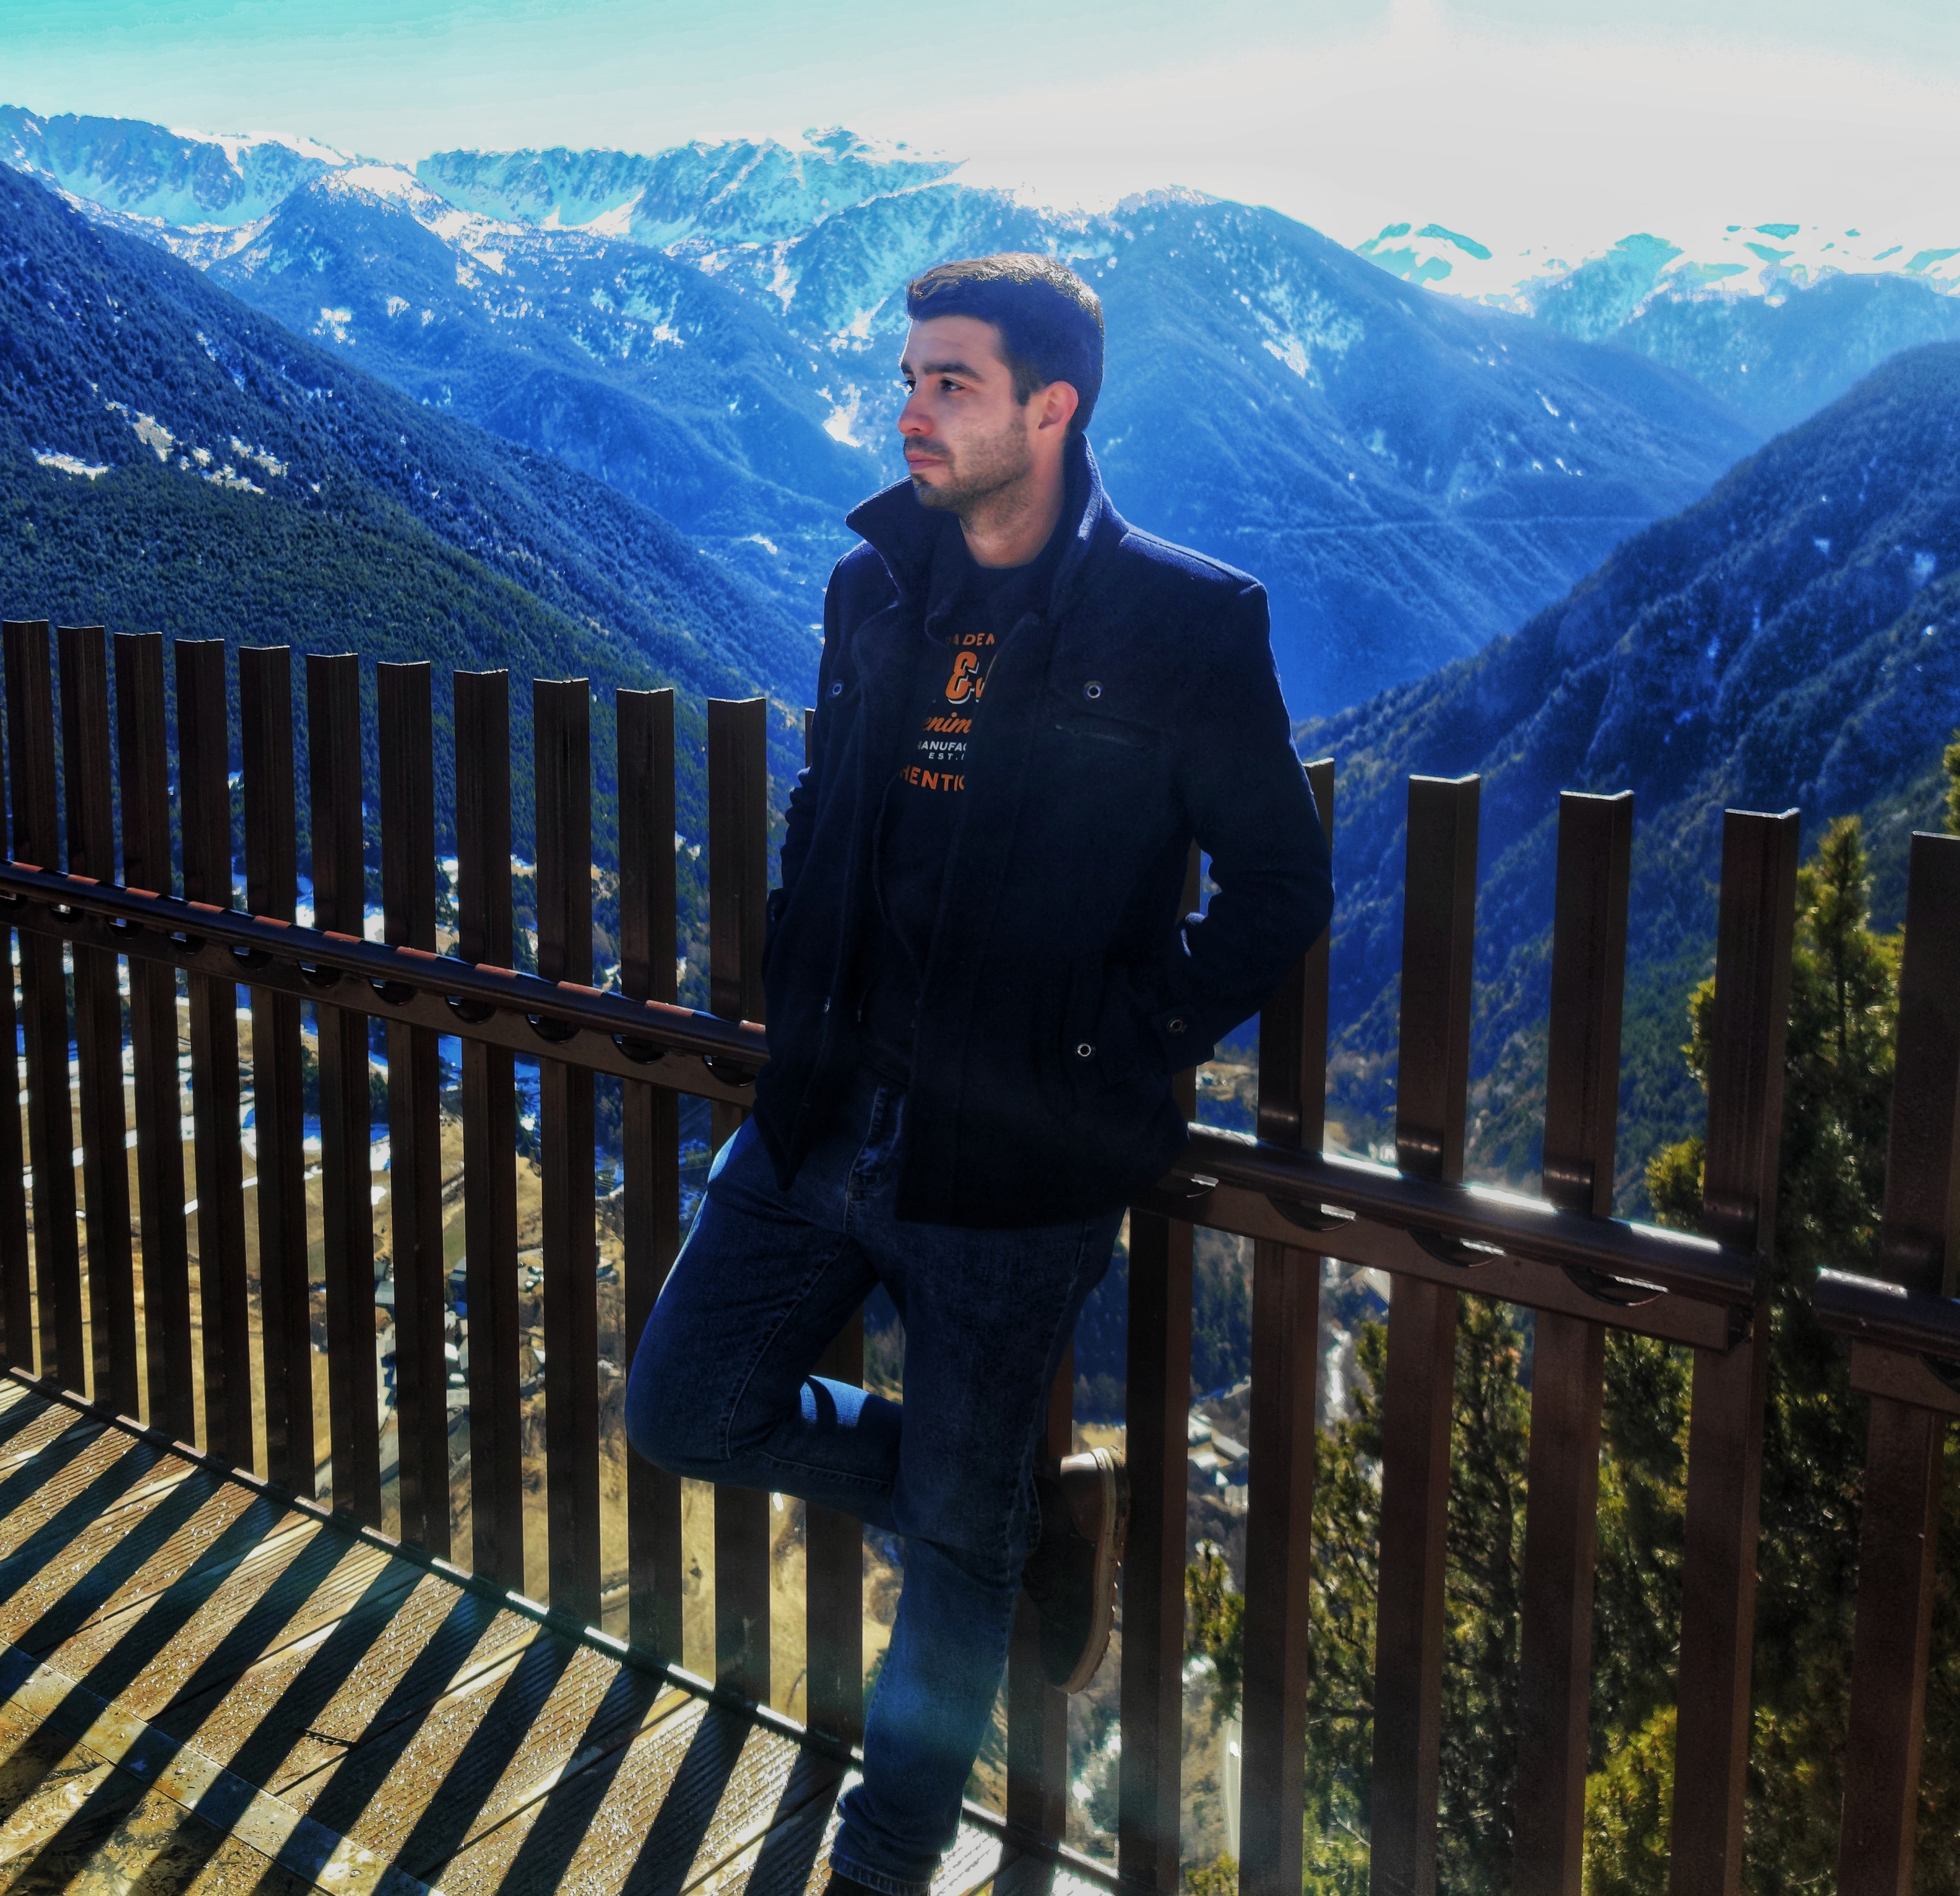
\includegraphics[width=5cm]{mifoto.jpg}};
	\end{tikzpicture}
	
	\vspace{4mm}

	{\Large \bfseries Miguel González Villa}

\end{center}

% \icontext{BirthdayCake}{14}{16/11/1994}{black}\\[6pt]
\icontext{MapMarker}{14}{Las Palmas de Gran Canaria}{black}\\[6pt]
\iconemail{EnvelopeO}{14}{miguel.gonzalez.villa@gmail.com}{miguel.gonzalez.villa@gmail.com}{black}\\[6pt]
% \icontext{Github}{14}{\href{https://github.com/yourid}{yourid}}{black}\\[6pt]
\icontext{Linkedin}{14}{\href{https://linkedin.com/in/miguel-gonzalez-villa}{LinkedIn}}{black}\\[6pt]
\icontext{Phone}{14}{+34 634 825 318}{black}\\[6pt]
%\cvqrcode{0.7}

%---------------------------------------------------------------------------------------
%	ABOUT ME
%----------------------------------------------------------------------------------------
\vspace{-8mm}

\section* {Sobre mi}

Amante de la cocina, videojuegos y el rock. De vez en cuando juego al baloncesto y trasteo con ordenadores.\\

\vspace{-2mm}

%---------------------------------------------------------------------------------------
%	META SKILLS
%----------------------------------------------------------------------------------------
% \cvsection{SKILLS}
% %\cvskill{Skill_Name} {Years of experience} {percentage of bar fill} \\[-2pt]

\section* {Habilidades}

\cvskill{Typescript} {7+ yrs} {1} \\[-6pt]

\cvskill{NodeJS} {7+ yrs} {0.9} \\[-6pt]

\cvskill{SQL} {5+ yrs} {0.9} \\[-6pt]

\cvskill{Análisis de datos} {4+ yrs} {0.7} \\[-6pt]

\cvskill{Integración continua} {2+ yrs} {0.4} \\[-6pt]

\cvskill{Gestión de equipo} {3+ yrs} {0.7} \\[-6pt]

\cvskill{Resolución de incidencias} {6+ yrs} {0.8} \\[-6pt]

% \cvskill{Cloud computing} {2+ yrs} {0.6} \\[-2pt]

\vspace{-2mm}
%\cvqrcode{0.7}

%---------------------------------------------------------------------------------------
%	EDUCATION
%----------------------------------------------------------------------------------------
%\vfill\null
% \cvsection{Educación}
\section*{Educación}

\begin{description}
	\raggedright
	\item [\normalfont \textcolor{ColorOne}{2018.}] \textbf{Grado en Ingeniería Informática}\\
	Universidad de Las Palmas de Gran Canaria\\
	%City -- COUNTRY
\end{description}

% \cvevent
% 	{\textbf{20XX - 20XX}}
% 	{M. Tech. - Computer Science $\&$ Engineering}
% 	{University Name - City, State (Country)}
% 	{Passed with \textbf{X.XX CGPA}. Thesis work on Your thesis domain.}
% \vfill\null

% \vspace{5mm}

%---------------------------------------------------------------------------------------
%	ACHIEVEMENTS
%----------------------------------------------------------------------------------------

% TODO: ESTO PARA GENERAR UNA NUEVA PÁGINA CON LO QUE CONLLEVA
% TODO: ESTO PARA GENERAR UNA NUEVA PÁGINA CON LO QUE CONLLEVA
% TODO: ESTO PARA GENERAR UNA NUEVA PÁGINA CON LO QUE CONLLEVA
\newpage

% \cvsection{ACHIEVEMENTS}

% \cvmetaevent
% {GATE}
% {Computer Science and Information Technology (CS)}
% {}
% {Qualified in 2016 with 389 score in general category.}

% \cvmetaevent
% {IELTS}
% {7.0 out of 9 Band}
% {}
% {A certificate issued by International Development Program (IDP), Australia to prove English language proficiency for non-native English language speakers.}

% \cvmetaevent
% {Cloud Computing 101}
% {94.30\%}
% {}
% {A certificate issued by coursera to prove basic understanding of cloud computing.}

\end{leftcolumn}
\begin{rightcolumn}
%---------------------------------------------------------------------------------------
%	TITLE  HEADER
%----------------------------------------------------------------------------------------
% \fcolorbox{white}{darkcol}{\begin{minipage}[c][3.5cm][c]{1\mpwidth}
% 	\begin {center}
% 		\HUGE{ \textbf{ \textcolor{white}{ \uppercase{ YOUR NAME } } } } \\[-24pt]
% 		\textcolor{white}{ \rule{0.1\textwidth}{1.25pt} } \\[4pt]
% 		\large{ \textcolor{white} {Research Scholar - Computer Science \& Engineering } }
% 	\end {center}
% \end{minipage}} \\[14pt]
% \vspace{-12pt}

%---------------------------------------------------------------------------------------
%	WORK EXPERIENCE
%----------------------------------------------------------------------------------------

\vfill\null
% \cvsection{Experiencia}
\section*{Experiencia}

\vspace{3mm}

\cvevent
	{\textbf{Mayo 2021 - actualidad}}
	{Software Application Developer}
	{IBM \& Metrica Consulting}
	{
		Puesto en una importante empresa de telecomunicaciones para el desarrollo de un asistente conversacional y diversas herramientas.
		Destaca la monitorización de datos en tiempo real, incluyendo gran variedad de métricas a medida que actualmente se toman como referencia.\\
		Desde 2024 colaboro en un proyecto para su fusión con otros operadores de telecomunicaciones, expandiendo aun más la capacidad de las herramientas mencionadas para abarcar alrededor de un 70\% más volumen de datos.\\
		Entre mis tareas también figuran:
	}
	{
		\cvlist{Diseño y desarrollo de APIs orientadas a entornos de alta disponibilidad, con despliegues en los sistemas de IBMCloud, Amazon EKS y Google Kubernetes Engine (GKE).}
		\cvlist{Desarrollo de aplicaciones web en TypeScript + Angular.}
		\cvlist{Gestión y desarrollo de un equipo, además de planificación de tareas.}
		\cvlist{Mantenimiento y mejora de aplicaciones destinadas al procesado autónomo de datos.}
		\cvlist{Gestión y uso de bases de datos PostgreSQL y Oracle.}
	}
\vfill\null

\vspace{5mm}

\cvevent
	{\textbf{Febrero 2018 - Abril 2021}}
	{Programador Junior}
	{Contactel Teleservicios - Grupo Inetel}
	{}
	{
		\cvlist{Desarrollo de aplicaciones web en Typescript + React + PostgreSQL sobre un servidor Express orientado al manejo de datos y alta disponibilidad.}
		\cvlist{Mantenimiento de aplicaciones en Java v8.}
		\cvlist{Soporte y resolución de incidencias de clientes en turnos de 24h junto a un equipo de desarrolladores.}
	}
\vfill\null
%---------------------------------------------------------------------------------------
%	PUBLICATION
%----------------------------------------------------------------------------------------
% \vspace{-0.5cm}
% \vfill\null
% \cvsection{PUBLICATIONS}

% \cvevent
% 	{\textbf{UGC Listed}}
% 	{Title of your research paper}
% 	{Journal Name (ISSN: XXXX-XXXX) Vol XX, Issue XX, 20XX}
% 	{Status: Accepted and Published}
% 	{}
% \vfill\null

% \cvevent
% 	{\textbf{SCI - IF X.XXX}}
% 	{Title of your research paper}
% 	{Journal Name (ISSN: XXXX-XXXX) Vol XX, Issue XX, 20XX}
% 	{Status: Under Review}
% 	{}
% \vfill\null

%---------------------------------------------------------------------------------------
%	PROJECTS
%----------------------------------------------------------------------------------------
% \vfill\null
% \cvsection{PROJECTS}

% \cvevent
% 	{\textbf{20XX}}
% 	{Project Name}
% 	{Tool: Python, Raspberry Pi}
% 	{A short description of your project.}
% \vfill\null

% \cvevent
% 	{\textbf{20XX}}
% 	{Project Name}
% 	{Tool: Web Development}
% 	{A short description of your project.}
% \vfill\null


%---------------------------------------------------------------------------------------
%	WORKSHOPS
%----------------------------------------------------------------------------------------
% \vfill\null
% \cvsection{WORKSHOPS \& CONFERENCES}

% \cvevent
% 	{\textbf{Mon 20XX}}
% 	{Name of Conference}
% 	{Conducted by}
% 	{}
% \vfill\null

% \cvevent
% 	{\textbf{May 2019}}
% 	{IEEE Internation Conference on Future of Internet of Things}
% 	{IEEE \& IIT Kanpur}
% 	{}
% \vfill\null

%---------------------------------------------------------------------------------------
%	SKILLS
%----------------------------------------------------------------------------------------

%---------------------------------------------------------------------------------------
%	PERSONAL DETAILS
%----------------------------------------------------------------------------------------
% \vfill\null
% \cvsection{EXTRACURRICULAR}
% \vspace{-0.3cm}
% \begin{itemize}
%   \item Put all the points that are not covered in \textbf{above sections}.
%   \item Put all the points that are \textbf{not covered} in above sections.
%   \item Put all the \textbf{points} that are not covered in above sections.
%   \item \textbf{Put all the points} that are not covered in above sections.
% \end{itemize}
% \vfill\null


% hotfixes to create fake-space to ensure the whole height is used
\vfill
\vfill
\vfill
\end{rightcolumn}
\end{paracol}
\end{document}